\documentclass{article}
\usepackage[slovene]{babel}
\usepackage[a4paper,top=2cm,bottom=2cm,left=3cm,right=3cm,marginparwidth=1.75cm]{geometry}
\usepackage{amsmath, amsthm, amsfonts, amssymb}
\usepackage{float}
\usepackage{graphicx}
\usepackage{mathtools}

\DeclareMathOperator{\se}{SE}
\DeclareMathOperator{\de}{p}
\DeclareMathOperator{\CM}{C}

\title{Projetkna naloga pri statistiki}
\author{Tadej Mohorčič}
\date{}

\begin{document}
    
    \maketitle

    Python datoteke z rešenimi nalogami lahko najedete na GitHubu: link.

    %%%%%%%%%%%%%%%%%%%%%%%%%%%%%%%%%%%%%%%%%%%%%%%%%%%%%%%%%%%%%%%%%%%%%%%%%%%%%%%%%%%%%%%%%%%%%%%%%%%%%%%%%%%%%%%%%%%%%%%%%%%%%%%%%%%%%%%%%%%%%%%%%%%%%%

    \section{Prva naloga}
    Pri tej nalogi smo obravavali $43886$ družin, ki živijo v mestu Kibergrad. Natančneje, morali smo obravnavati delež družin, kjer glava družine nima srednješoljske izobrazbe,
    to pa bomo storili z enostavnim vzorčenjem in ocenjevanjem. Med podatke smo dodali spremenljivko, poimenovano \textbf{Brez Izobrazbe}. Ta je indikator dogodka, ali imamo
    srednješolsko izobrazbo ali ne, torej ima vrednosti le 0 in 1. Tukaj smo vrednost 1 dodelili tistim družinam, kjer glava nima srednješoljske izobrazbe. Nekatere podatke sem
    zbral v tabeli Data200 in Data800.

    \subsection{A del naloge}
    Tukaj smo vzeli naključno izbran delež 200 družin iz celotne populacije. Kot oceno za delež populacije smo tako vzeli kar delež na tem naključno izbranem vzorcu.
    \par \textbf{Ocena za delež je 0.205.}

    \subsection{B del naloge}
    Oceno za standardno napako najdemo s formulo
    \[
        {\widehat{\se}_{+}}^2 = \sqrt{\frac{(N - n)\de(1 - \de)}{(n - 1)N}}
    \]
    kjer je $N$ velikost populacije, $n$ velikost vzorca, $\de$ pa je populacijski delež. Za $\de$ tukaj uporabimo rezultat iz prejšnje naloge. Za interval zaupanja pa lahko
    vzamemo kar $\de \pm 1.96{\widehat{\se}_{+}}^2$.
    \par \textbf{Standardna napaka je 0.0299879137.}
    \par \textbf{Interval zaupanja je (0.1671131677, 0.2992038693).}

    \subsection{C del naloge}
    Pravi populacijski delež in pravo standardno napako najdemo kar z uporabo funkcij .mean() in .var().
    \par \textbf{Pravi populacijski delež je 0.2115025293.}
    \par \textbf{Prava standardna napaka je 0.0288767216.}
    \par \textbf{Interval zaupanja pokrije pravi populacijski delež.}

    \subsection{D del naloge}
    \begin{figure}[H]
        \begin{center}
            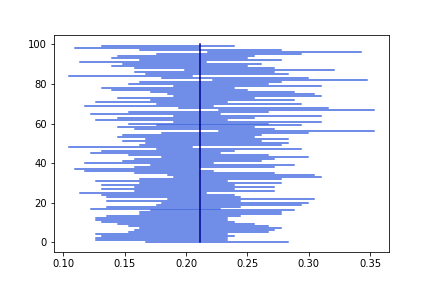
\includegraphics[scale=0.5]{../Python Koda/IZ200.png}
            \caption{IZ za 100 vzorcev velikosti 200 družin}
            \label{200}
        \end{center} 
    \end{figure}
    Tukaj smo morali zgenerirati še 99 vzorcev velikosti 200, in za vsakega izračunati interval zaupanja, ti pa so prikazani na sliki \ref{200}.
    \par \textbf{92 intervalov zaupanja pokrije populacijski delež.}

    \subsection{E del naloge}
    Standardni odklon vzorčnih deležev izračunamo kar z .std(), standardno napako za vzorec velikosti 200 pa po enaki formuli kot prej, le da vstavimo v formulo populacijski delež.
    Pri primerjavi pride do zelo majhnega odstopanja, zato bi rekli da je standardni odklon primerljiv z standardno napako za vzorec velikosti 200.
    \par \textbf{Standardni odklon je 0.0297648702.}
    \par \textbf{Standardna napaka za vzorec velikosti 200 je 0.0288828163.}

    \subsection{F del naloge}
    Zadnji dve točki smo morali ponoviti še za vzorce velikosti 800. Do rezultatov pridemo po isti poti kot zgoraj.
    \begin{figure}[H]
        \begin{center}
            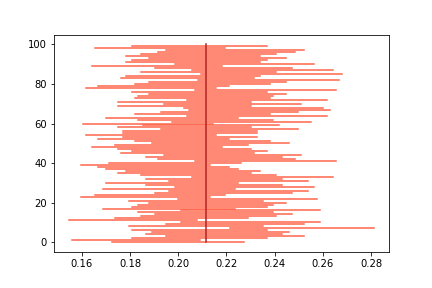
\includegraphics[scale=0.5]{../Python Koda/IZ800.png}
            \caption{IZ za 100 vzorcev velikosti 800 družin}
            \label{800}
        \end{center} 
    \end{figure}
    Intervali zaupanja so za večji populacijski delež precej bolj skoncentrirani ob sredini, prav tako pa so tudi ožji, kar lahko razberemo iz tabele Data800. Opazno pa je
    tudi standardni odklon precej manjši, in tudi bližji pravi standardni napaki za vzorev velikosti 800. Verjetno se bosta ti dve vrednosti še bolj zbližali, če velikost vzorca
    pošljemo proti večji številki.
    \par \textbf{97 intervalov zaupanja pokrije populacijski delež.}
    \par \textbf{Standardni odklon je 0.0141844710}
    \par \textbf{Standardna napaka za vzorec velikosti 800 je 0.0143149434.}

    %%%%%%%%%%%%%%%%%%%%%%%%%%%%%%%%%%%%%%%%%%%%%%%%%%%%%%%%%%%%%%%%%%%%%%%%%%%%%%%%%%%%%%%%%%%%%%%%%%%%%%%%%%%%%%%%%%%%%%%%%%%%%%%%%%%%%%%%%%%%%%%%%%%%%%

    \section{Druga naloga}
    Pri tej nalogi smo obdelali odčitane telesne temperature pri moških in pri ženskah, kjer smo privzeli da sta za oba spola ti vrednosti porazdeljeni normalno.

    \subsection{A del naloge}
    Za oceno povprečja in standardnega odklon lahko uporabimo kar funkciji .mean() in .std(). Vemo, da je povprečje na vzorcu dobra cenilka za povprečje, medtem ko funckija
    .std() zraven še upošteva faktor $\frac{1}{N - 1}$, za katerega pa tudi vemo, da je nepristranska cenilka.
    \par \textbf{Povprečje je 36.7247863248 pri moških in 36.8854700855 pri ženskah.}
    \par \textbf{Standardni odklon je 0.3881976457 pri moških in 0.4130487515 pri ženskah.}

    \subsection{B del naloge}
    Za obe povprečji smo morali doložiti 95\% interval zaupanja. V šoli smo pokazali, da če $\sigma$ ni znan (pri nas ne poznamo točne vrednosti), potem za X, ki je
    porazdeljen normalno, velja
    \[
        \frac{\overline{X} - \mu}{\widehat{\sigma}^{+}} \sqrt{n} \sim Student(n - 1)
    \]
    Tako bomo tukaj morali namesto funkcije napake erf uporabiti funkcijo Studentove porazdelitve. Kalkulator na spletu nam vrne, da je za 95\% zaupanja pri 64 prostorskih stopnjah
    vrednosti $1.9977$. Dobimo, da je 
    \[
        \CM_{\alpha} = 1.9977\frac{\widehat{\sigma}^{+}}{\sqrt{n}}
    \]
    \par \textbf{Interval zaupanja za moške je (36.6285970859, 36.8209755637).}
    \par \textbf{Interval zaupanja za ženske je (36.7831231354, 36.9878170355).}

    \subsection{C del naloge}
    Sedaj pa moramo testirati domnevo, da imajo moški in ženske v povprečju enako telesno temperaturo. Imamo torej $M_{1}, \ldots, M_{65}$ in $Z_{1}, \ldots, Z_{65}$ porazdeljeno
    normalno z $\mu_{M}$ in $\mu_{Z}$ ter testiramo:
    \begin{itemize}
        \item $H_{0}$: $\mu_{M} = \mu_{Z}$
        \item $H_{1}$: $\mu_{M} \neq \mu_{Z}$
    \end{itemize}
    Na vajah smo pokazali, da za spremenljivko T velja
    \[
        T \coloneqq \frac{\overline{X} - \overline{Y}}{S}\sqrt{\frac{mn}{m + n}} \sim Student(n + m - 2),
    \]
    kjer je
    \[
        S \coloneqq \sqrt{\frac{\sum_{i = 1}^n (X_{i} - \overline{X})^2 + \sum_{i = 1}^m (Y_{i} - \overline{Y})^2}{m + n - 2}}.
    \]
    Pri nas je $m = n = 65$, $X$ in $Y$ pa sta ravno odčitane vrednosti temperature moških in žensk. Z uporabo formule
    \[
        P(|\overline{M} - \overline{Z}| \leq \CM_{\alpha}) \leq \alpha 
    \]
    dobimo rezultate. Ker je $|\overline{M} - \overline{Z}| = 0.1606837607$, bomo domnevo obdržali le pri 0.01\% stopnji tveganja.
    \par \textbf{Pri stopnji tveganja 0.05\% je interval (-0.1391179454, 0.1391179454).}
    \par \textbf{Pri stopnji tveganja 0.01\% je interval (-0.1838407053, 0.1838407053).}
\end{document}